\documentclass[a4paper,twocolumn]{esapub2005} % European paper
\pagestyle{empty}
\bibliographystyle{alpha}
\usepackage{times}
\usepackage{natbib}
\usepackage{tikz}
\usepackage{graphicx}

\title{Seemless Integration of Reconfigurable Hardware into the Robotic Development Process}
\author{Moritz Schilling}
\affil{DFKI GmbH, Robert-Hooke-Str. 5, 28359 Bremen, Germany}
\affil{TEC-MMA, ESTEC, 2200 AG Noordwijk, The Netherlands}

\newcommand{\btx}{\textsc{Bib}\TeX}

\begin{document}

\maketitle

\begin{abstract}
Modern robotic development frameworks have agreed upon the model-based, component-centric software development approach. Composing robotic control software has become an easier and less error-prone task. While there is a model for the software architecture and – fairly recently – a model for the kinematical structure of robotic systems, models for other aspects are missing. This paper will focus on the model of heterogeneous computational resources and their interconnection within a robot and outline how tools make use of the models to generate code skeletons in different languages, find compatible implementations of algorithms given a specific target and to map a network of software to a network of hardware components.
\end{abstract}

% Introduction/Motivation

\section{Introduction}

Robotic systems are becoming more and more complex either in mechanical, electronic or software domain.
Regarding electronic and software domain this complexity mainly arises from the composition of different, heterogeneous processing devices and their interconnections.
How this heterogeneity in hardware can be transformed to homogeneity in the software domain has gained much attention in research - but mostly outside of the robotics community.
As robotic systems are also distributed, heterogenous, embedded systems the development of robot control systems will benefit from these research efforts.
For example, the development process itself will be accelerated, the usage of ressources will be more efficient and/or the robustness of the system against failure will increase.

While there has been much progress in unifiing the programmability of networks of heterogeneous, conventional computing devices,
reconfigurable hardware devices (e.g. Field Programmable Gate Arrays) still have to be treated seperately.
How such devices can be seemlessly incorporated into existing robotic development frameworks which have been developed to improve the re-usability of software and to ease the programming of robotic systems is the main focus of this research.
Such a framework shall be enabled to make use of the advantages of reconfigurable hardware, while maintaining system stability, integrity and predictability.

%The idea is to provide a library of reusable software components with defined functionality and interfaces such that the user only needs to group and interconnect them to setup a robotic system.
%Then the framework takes care of providing glue code for the interaction of the components, for possible data transfer as well as the deployment onto the target system.
% SotA
% Gaps
%\section{Current Approaches}
In the following a review of the state of the art with respect to the programming of heterogeneous processing devices in embedded systems like robots is presented. Besides robotic development frameworks a look into other related areas of research is taken as well.

The considered frameworks have been selected either because of their popularity amongst the robotics community or because they exhibit an outstanding feature:
\begin{description}
    \item[ROCK] the Robot COnstruction Kit which is mostly used by DFKI and ESTEC and runs on robots like SpaceClimber, SpaceBot or Asguard\cite{ROCK},
    \item[BG] the Behaviour Graphs which have been recently developed at DFKI to model the reactive layer of robots like SpaceClimber or Charlie\cite{2012_Langosz},
    \item[ADE] a framework from the University of Notre Dame which has been used to control the famous Nao robots\cite{Scheutz},
    %\item the Player/Stage framework from the University of Auckland which is supported and used by many robots and groups worldwide,
    %\item the Miro framework from the University of Ulm which has been used to run Pioneer robots or the B21,
    \item[GenoM3] the Generator of Modules toolset developed at LAAS-CNRS and is used to design real-time software architectures in the robotic and space domain\cite{2015_Genom3},
    \item[ROS] the Robot Operating System which is one of the most popular frameworks in the robotics community\cite{ROS}, and
    \item[LabView] which is not a pure robot development framework but has been used for this purpose\cite{2010_Muecke}.
\end{description}
These frameworks are analysed with respect to
\begin{itemize}
    \item Component model and granularity,
    \item Execution semantics,
    \item Transparency,
    \item Portability across processing device families, and
    \item Hardware modelling capabilities.
\end{itemize}

% ESA-NPI Meeting with Gianfranco:
% * Add GenoM to list of FWs
% * Clearly differentiate what is your own contribution!
% * Look at it like a daisy (?) (DROCK <-> ESA NPI)
% * Regular exchange of status with Gianfranco
\subparagraph{Component Model and Granularity}
This property is about the interfaces a component comprises to the developer.
The interface defines which \emph{data types} are used and what the \emph{types of the ports} are.
%Additionally, the frameworks can also exhibit a restriction on the granularity of the most basic components (atomic components).
The granularity of the basic components might also be a distinctive feature of robotic development frameworks, even if there are no imposed restrictions.

\subparagraph{Execution Semantics}
\begin{figure}
    \centering
    %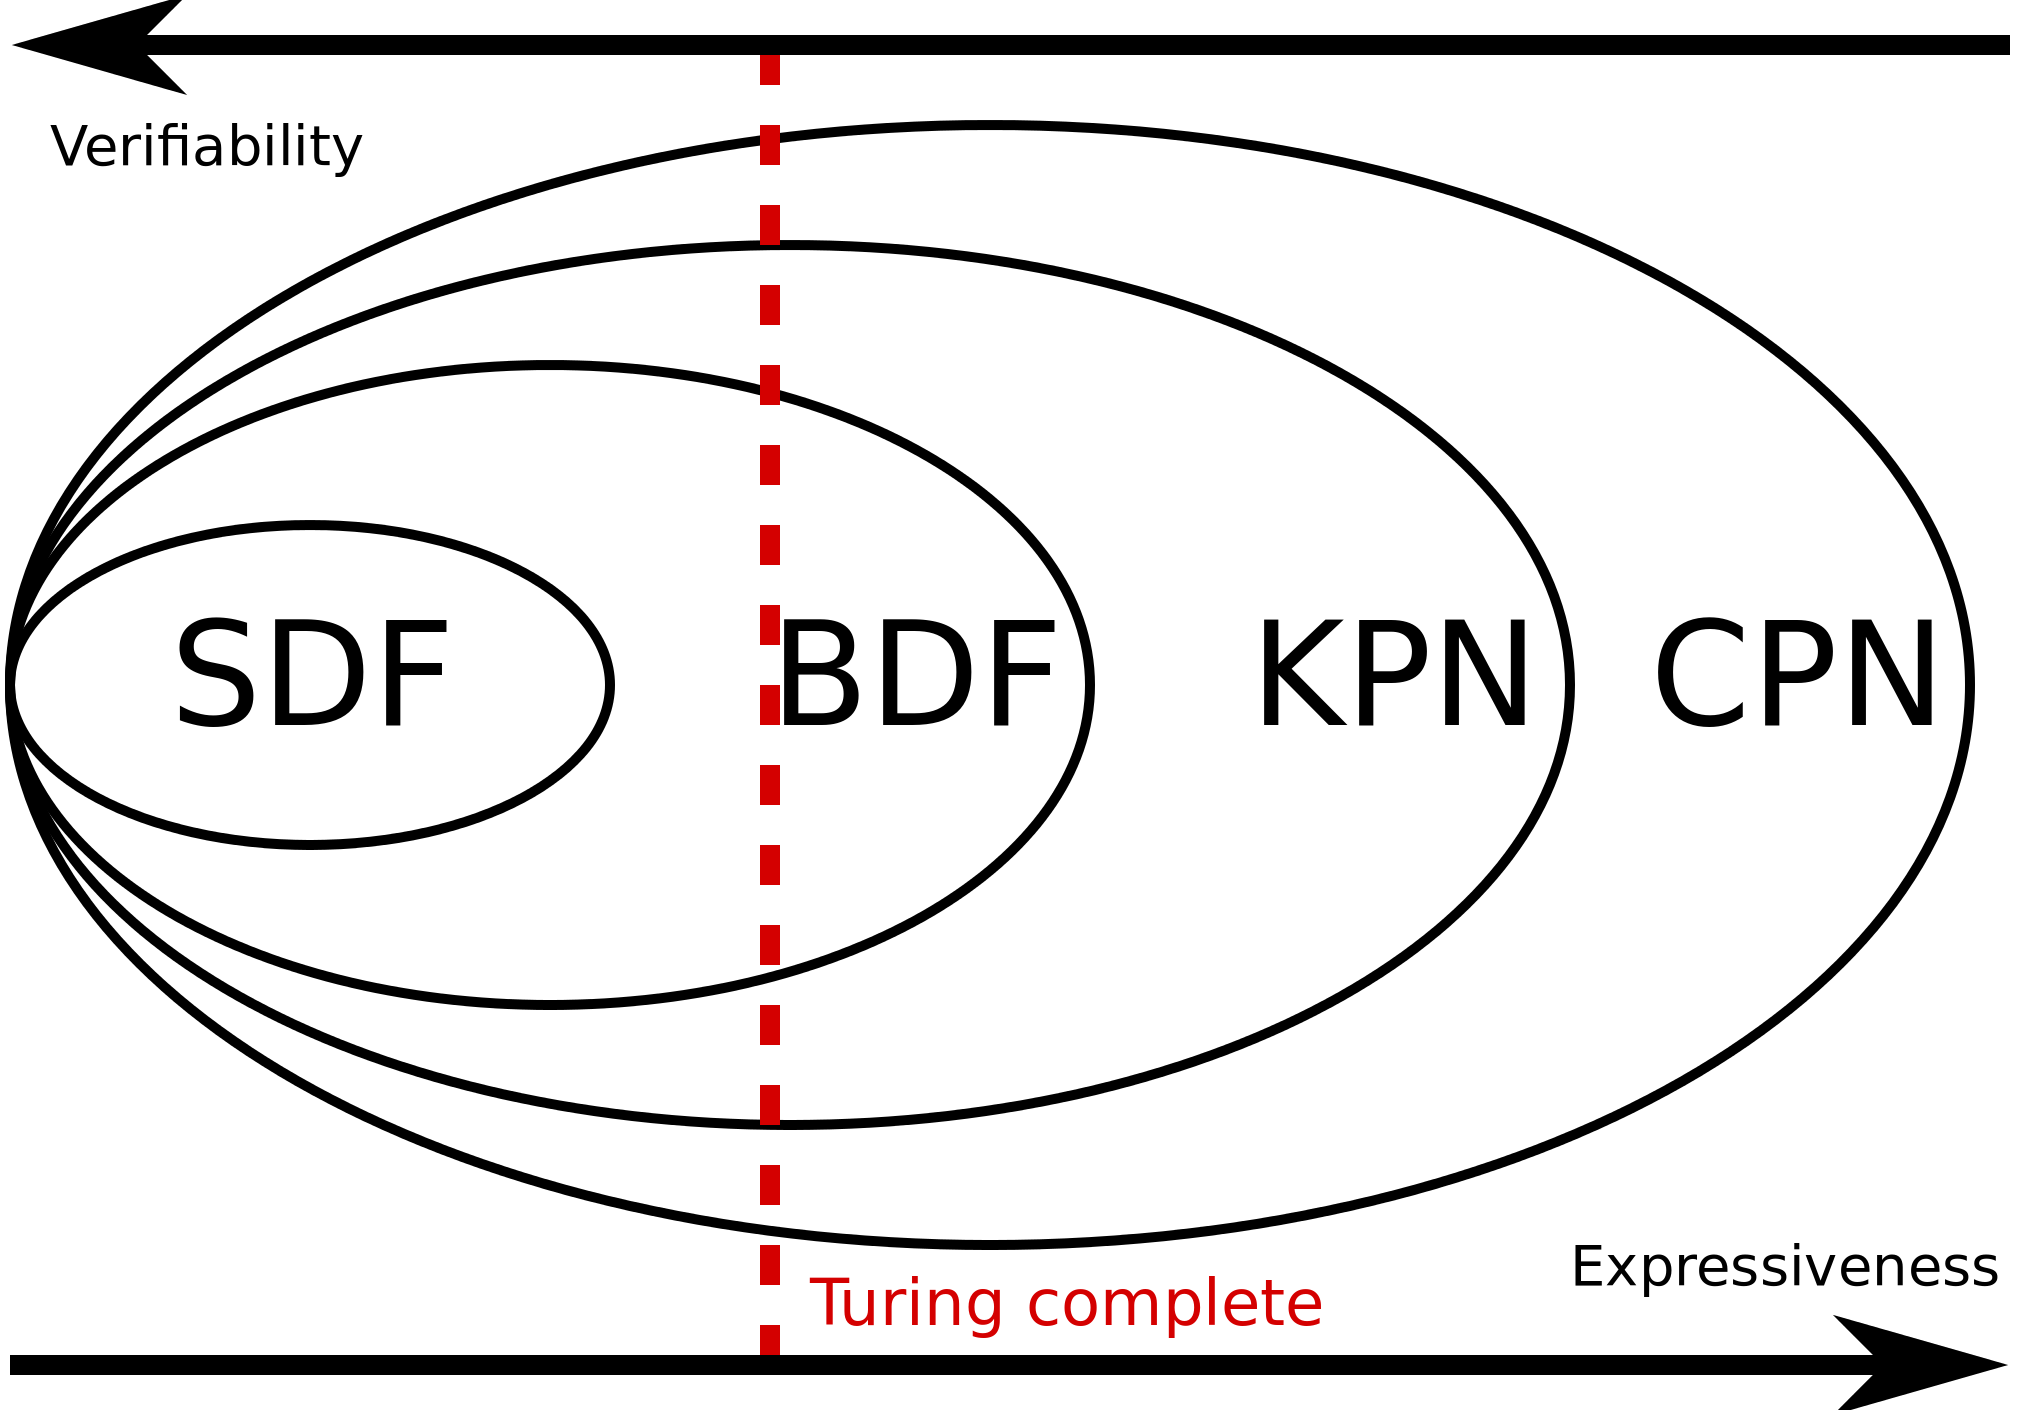
\includegraphics[width=0.5\textwidth]{pics/Verification.png}
    \caption{
        The relationship between verifiability and expressiveness for a selection of computational models.
        BDF stands for Boolean Dataflow and extends the SDF domain with data-dependent routing capabilities.
        Based on \cite{Basten}.
    }
    \label{fig:verifiability}
\end{figure}
This property specifies under what conditions a component is to be executed.
It is closely related to the \emph{model of computation} which the framework follows.
At the one extreme there are \emph{decidable}, \emph{deterministic} models of computation
while on the other end there are \emph{undecidable}, \emph{nondeterministic} models.
To get a categorization, three well-known models have been chosen:
\begin{description}
    \item[SDF] Static Data Flow (decidable and deterministic)
    \item[KPN] Kahn Process Networks (undecidable and deterministic)
    \item[CPN] Coloured Petri Nets (undecidable and nondeterministic)
\end{description}
The execution model directly influences the possibility of verification and the expressiveness of the component networks.
The more expressive the less verifiable such a network becomes.
%Buck has found the border at which a model becomes turing-complete\cite{1993_BDF} and therefore undecidable in general.
Figure \ref{fig:verifiability} visualizes this relationship.

\subparagraph{Transparency}
Transparency specifies which implementation details are hidden from the user such that he doesn't need to care about.
\begin{description}
\item[Communication] transparency hides the details of data transport from the user,
\item[Transaction] transparency hides the coordination of dependent components from the user,
\item[Location] transparency hides the location of a component in the system from the user,
\item[Migration] transparency hides the relocation of components in execution from the user,
\item[Replication] transparency hides the cloning of components from the user,
\item[Ressource] transparency hides the ressource management from the user,
\item[Persistence] transparency ensures that the creation/destruction of components do not affect independent components,
whereas \item[Failure] transparency hides the failure and recovery of components during execution.
\end{description}
A detailed and formal description of these transparencies can be found at \cite{RM-ODP}.

\subparagraph{Portability}
Because this project is about distributed, \emph{heterogeneous} systems, the frameworks have to be analysed with respect to their support of different processing devices.
Hereby, it is of special interest if the frameworks not only support conventional processing devices - like \emph{CPU}s or \emph{$\mu$C}s - but also support reconfigurable hardware, namely \emph{FPGA}s.

\subparagraph{Hardware Modelling}
%Portability is only one aspect of the programmability of distributed systems.
%The other one is the modelling of the computational infrastructure.
The frameworks are analysed with respect to their modelling capabilities of \emph{sensors}, \emph{actuators}, \emph{computational resources} and \emph{network topology}.
These capabilities are essential for distributed systems support.
Other important modelling capabilities like mechanical structure, kinematics etc. are neglected here.

%\subparagraph{Evaluation}
ROCK components comprise an interface consisting of inputs, outputs and parameters (properties) with data types derived from C++ types.
Furthermore, components have and publish their state of execution which can be controlled by the user.
The components are mostly coarse-grained (containing complete subsystems/algorithms) although granularity is arbitrary in general.
Semantics roughly follow the KPN model; components are connected peer-to-peer through channels and are accessed by read/write functions.
However, the user can (but shouldn't) circumvent the KPN model because emptiness of a channel can be tested.
ROCK uses message queues or CORBA for data transport dependent on the location of the interacting components.
To some extend there are mechanisms to automatically restart components on failure.
Components can be deployed to systems with conventional, high-performance processing devices capable of hosting a UNIX OS.

Behaviour Graph components (nodes) exhibit inputs and outputs with C float type.
The granularity of the atomic components is fine-grained; they are pure mathematical operators (like add, multiply etc.).
As such, their semantics follow the SDF model.
Only if all of their operands are available operations are executed.
Currently, behaviour graphs can only be executed on CPUs or $\mu$Cs and only the coordination of the components is hidden from the user.

ADE components have four types of interface links,
\begin{itemize}
    \item activation links,
    \item observation links,
    \item process control links, and
    \item component links.
\end{itemize}
Activation links are used to exchange data between components,
observation links pass state information to other components while process control links can change state,
and component links allow components to create new components.
Because of these properties the semantics of a component follow the CPN model in which non-determinism is allowed.
Communication relies on registries, servers and clients and is implemented in JAVA language as well as the components itself.
Therefore, an ADE component needs a JAVA virtual machine on top of conventional processing device (and possibly an OS).
This virtualization and the component link mechanism provide replication transparency.
Although it would be possible, migration transparency is not yet a property of ADE.
ADE also models computational structure of the system in form of virtual machines connected by communication links.

A GenoM3 component consists of inputs and outputs of data types defined in the Interface Description Language of CORBA.
Additionally, it defines events which are used e.g. to change state of the component.
The component behaviour is directly modeled as a Petri Net; so the semantics is of the CPN domain.
GenoM3 uses middleware templates to specify the glue code neccessary for communication, distribution etc.
Therefore, all other properties strongly depend on these templates.
For example, a VHDL template could be developed which would enable GenoM to support reconfigurable hardware.

ROS components do not have the notion of inputs and outputs but use the concept of topics.
Topics are anonymous channels to which a ROS component can subscribe to or to which it can publish information.
As such, components are not directly coupled as in statically defined component networks.
Instead, they form a component network at run-time.
This process enables non-deterministic behavior because it is not known which component is connected to which of the others beforehand.
%Even during runtime the topology of the component network can change arbitrarily.
The semantics are therefore of the CPN domain.
As most of the previously presented frameworks, ROS also provides glue code for communication etc.

Although LabView is not a robotic development framework of its own, it has been used for this purpose.
The components of LabView follow the SDF semantics like those of the Behaviour Graph framework.
But the available components allow much more than purely mathematical operators; there are also components which exhibit data-dependent behaviour like loops and if-then-else structures.
LabView also provides the necessary glue code to let the components interact and it is the only framework considered here which is able to deploy them to FPGAs.
However it remains unclear if distributed operation in heterogeneous processing networks is supported by the toolchain.

%\paragraph{Identified Gaps and Delta}
%TODO: Verify table contents!!!!
\begin{table*}
    \centering
    %\resizebox{0.5\textwidth}{!}{
    \begin{tabular}{l|cccccc}
        Framework & Interface & Granularity & Semantics & Transparency & Portability & Models \\
        \hline
        ROCK & C types & Coarse & KPN & Communic. & CPU & Sensor\\
             & Inputs  &        &     & Failure       & UNIX      & Actuator \\
             & Outputs &        &     & Transaction   &           & \\
             & Parameter &      &     & Location      &           & \\
             & State   &        &     & Ressource     &           & \\
             &         &        &     & Persistence   &           & \\
        \hline
        Behaviour & C float & Fine & SDF & Transaction & CPU & \\
        Graphs    & Inputs  &      &     &             &     & \\
                  & Outputs &      &     &             &     & \\
        \hline
        ADE  & C types & Coarse & CPN    & Communic. & CPU & Sensor\\
             & Inputs  &        & (Client/ & Persistence  & JVM & Actuator \\
             & Outputs &        & Server) & Transaction   &          & Comp.\\
             & Parameter &      &        & Replication   &          & Ress.\\
             & State     &      &        & Location      &          & Topology\\
             & Priority  &      &        & Ressource     &          & \\
             &         &        &     & Failure &           & \\
        \hline
        GenoM3 & IDL types & Coarse & CPN & Depends & Depends & Depends \\
               & Inputs    &      &     &           &       & \\
               & Outputs   &      &     &           &         & \\
               & Events    &      &     &             &     & \\
               & State     &      &        &               &          & \\
               & Priority  &      &        &               &          & \\
        \hline
        ROS    & IDL types & Coarse & CPN      & Communication & CPU & Sensors\\
               & Topics    &        & (Publish/ & Transaction   &     & Actuators\\
               &           &        & Subscribe, &             &     & \\
               & Parameter &        & Client/  &               &     & \\
               &           &        & Server)  &               &     & \\
        \hline
        LabView & Inputs   & Fine   & SDF & Communication & CPU  & Sensors\\
                & Outputs  &        &     & Transaction   & FPGA & Actuators\\
    \end{tabular}
    %}
    \caption{
        Evaluation of the different frameworks with respect to defined properties/features.
    }
    \label{table:summary}
\end{table*}
Table~\ref{table:summary} summarizes the properties of the different frameworks.
Most frameworks exhibit a very powerful and expressive component model while only ROCK, Behaviour Graphs and LabView use a more restrictive one.
As has been stated, more expressiveness comes at the price of less verifiability.
Although Behaviour Graphs and LabView applications could be verified the necessary tools for them are still missing.
When it comes to critical applications like space robotics this aspect can not be neglected.

Modern robots do not consist of homogeneous processing networks; in general they contain FPGAs, microcontrollers and full-blown CPUs.
The latter ones are architecturally similar but different in processing and storage capabilities.
At least they can share the same programming language base like C; this is not the case for FPGAs.
Only one of the frameworks supports the deployment of the same application to either a conventional target or an FPGA.

To be able to distribute a given application to more than one target in a processing network the topology of it has to be modeled.
To the knowledge of the author only ADE considers this model for distributing applications.
Furthermore, ADE allows dynamical redistribution during run-time which is the prerequisite to guarantee robustness against failures and load balancing.

None of the frameworks exhibits all of the properties neccessary for the programming of heterogeneous and distributed robotic systems which are
\begin{itemize}
    \item distributed computation
    \item verifiability
    \item heterogeneous processing networks
    \item dynamic reprogramming (not reconfiguration via parameter updates)
\end{itemize}

HERE IS SOMETHING MISSING!!!

%\paragraph{Related Research}
%\begin{itemize}
    %\item Partial Reconfiguration, Scrubbing
    %\item Virtualization, Middleware
    %\item HW/SW design languages (SIGNAL, Lustre)
    %\item Architecture Description Languages/Frameworks (BIP, AADL\cite{2015_Online_CMU})
    %\item Verification
%\end{itemize}
%\todo[inline]{ref to BIP}
%Some of the features needed to program a distributed, heterogeneous robotic system have been tackled within other areas of research.
%For example, the question of how to describe and model a system from both, the hardware and software perspective, is part of the development of architecture description languages/frameworks.
%Two prominent candidates in this field are the Behaviour Interaction Priority (BIP)\cite{2006_BIP} framework and the Architecture Analysis and Design Language (AADL)\cite{2015_Online_CMU}.
%Both of them allow to model the systems software by interacting component networks which is the same approach as in state-of-the-art robotic development frameworks.
%But, additionally, their component model follows a formal semantic such as to support timing analysis and verification.
%They also provide a model of the hardware components, e.g. processors, busses or memory, to which the software has to be deployed.
%Hoewever, none of them currently supports exotic targets like FPGAs.
%The TASTE toolset from ESA\cite{2012_TASTE} uses AADL in addition to other languages to support the programming of distributed, embedded real-time systems.
%Especially target architectures with devices of limited capabilties are addressed and even some basic FPGA support (by the means of accelerators) exists.
%But reconfigurable hardware is not equally treated as other, conventional devices of a robotic system.

%To be able to manage different targets to be programmed by a framework there has to be a mechanism which abstracts the details of underlying hardware.
%For conventional targets this task is mainly performed by the operating system or a virtual machine.
%On the other hand, unusual targets like FPGAs have no notion of an operating system and are programmed very differently from conventional ones.
%The HW/SW design languages like SIGNAL\cite{1991_Signal} can be used to develop software for all of these targets.
%Programs written in these languages can be easily verified because of the strict semantical models.
%The distribution of a given SIGNAL program given a simplified model of processors has been studied theoretically;
%the generated code is mainly intended for functional simulation\cite{2010_Signal}.

%The operating system BORPH\cite{2007_Borph} extends the UNIX process model to handle tasks on reconfigurable targets.
%It provides the necessary glue-code to connect the state of a hardware process to the state of a stub UNIX process.
%In contrast to the previously mentioned HW/SW design languages, BORPH handles the interconnection between individual software parts.
%But it does not provide abstraction; an expert has to design the hardware process itself before it is usable in BORPH.

%The TensorFlow\cite{2015_TensorFlow} framework can be used to define and distribute deep-learning neural networks to large-scale distributed systems.
%Although the framework makes use of graphical processing units (GPUs) the target architecture has to be homogeneous.
%All architectural entities have to have a conventional processing device and a hosting operating system to be manageable by TensorFlow.

%\paragraph{Summary}
%\begin{figure}
%    \centering
    %\includegraphics[width=0.7\textwidth]{pics/SotA_summarized.pdf}
%    \caption{
%        Schematic overview of the current state in robotic development frameworks and related areas of research.
%        The SIGNAL language and its toolset is an example of a framework supporting many heterogeneous processing devices including reconfigurable hardware devices.
%        At the other extreme, frameworks for deep-learning software like TensorFlow do not support processing devices like FPGAs
%        but support the distribution of an application to large-scale processing networks.
%    }
%    \label{fig:sota}
%\end{figure}

%Figure~\ref{fig:sota} summarizes the state-of-the-art of the robotic development frameworks embedded into the related areas of research.
%Currently, these frameworks do not model the system's processing and communication architecture,
%so the distributedness of control and the heteroegeneity of processing both are rather low.
%The SIGNAL language and its toolset are an %example of a framework supporting many %heterogeneous processing devices including %reconfigurable hardware devices.
%At the other extreme, frameworks for deep-%learning software like TensorFlow do not support %processing devices like FPGAs
%but support the distribution of an application in %large-scale processing networks.

%During the course of this activity the field of robotic development frameworks shall be extended to a domain with both, increased distributedness of the control software as well as
%better support of various, different processing devices - including reconfigurable hardware - found in modern robotic systems.

% This Approach
\section{Ontologies \& Beyond}
To overcome the lack of support for heterogeneous \& distributed systems, an additional modelling domain has to be incorporated into the development process.
Besides software components there are also hardware components like execution units and hardware architecture established by communication links.
Once this domain exists, a framework can exploit this to distribute the overall application to the robotic hardware.

HERE  IS SOMETHING MISSING!!!

% Hypergraph
THE FOLLOWING TEXT IS QUITE SHITTY!!!
First of all, the modelling domains are founded on common ground; this common ground is based on generalized hyperedges forming hypergraphs, sets \& relations formed from hyperedges and general, predefined relations forming hierarchies.
Generalized Hyperedges are edges which can link to other edges as well - unlike 'normal' hyperedges.
The predefined relations are
\begin{description}
    \item[\textbf{memberOf}] forming the concept of sets,
    \item[\textbf{isA}] forming a subsumption hierarchy,
    \item[\textbf{partOf}] forming a compositional hierarchy,
    \item[\textbf{has}] introducing the concept of ownership and aggregation, and
    \item[\textbf{instanceOf}] to distinguish the model from its instantiation/use.
\end{description}
The hypergraph/-edge concept allows the easy storage of different modelling domains and a formal definition of a query in all these domains as graph traversals through these domains.
In contrast to ordinary graphs, relations between sets have a natural representation in the form of generalized hyperegdes without the need of reification (making artificial entities to allow relations point to relations).

% Derived Domains
%   Hardware
%     Computational
%     TODO: Electrical
%     TODO: Kinematical
%   Software
%     Algorithm
%     TODO: FSM
%   Mixed
%     TODO: Implementations
%     TODO: Deployments
Based on this fundamental model, both domains \emph{hardware} and \emph{software} are derived.
\begin{figure}
    \centering
    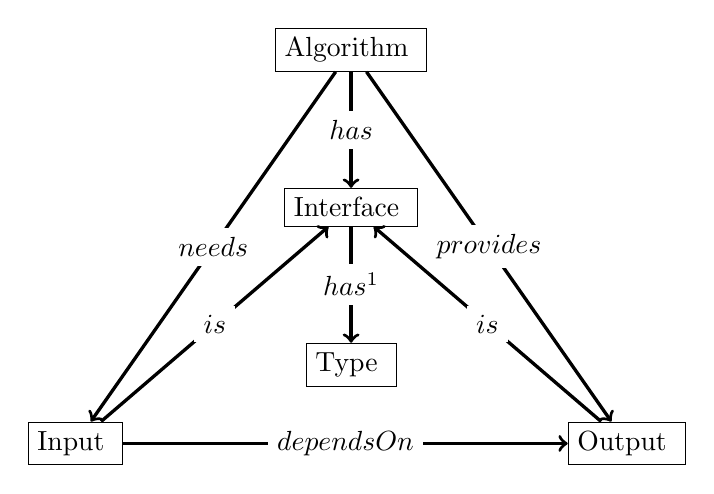
\begin{tikzpicture}
        \node[draw, align=center] (Algorithm) at (2,2.5) {
            Algorithm
        };
        \node[draw, align=center] (Interface) at (2,0.5) {
            Interface
        };
        \node[draw, align=center] (Type) at (2,-1.5) {
            Type
        };
        \node[draw, align=center] (Input) at (-1.5,-2.5) {
            Input
        };
        \node[draw, align=center] (Output) at (5.5,-2.5) {
            Output
        };
        %\node[draw, align=center] (Dependency) at (3,-3.5) {
        %    Dependency
        %};
        \draw[->, very thick] (Algorithm) to node[fill=white] {
            $has$
        } (Interface);
        \draw[->, very thick] (Interface) to node[fill=white] {
            $has^1$
        } (Type);
        \draw[->, very thick] (Algorithm) to node[fill=white] {
            $needs$
        } (Input);
        \draw[->, very thick] (Algorithm) to node[fill=white] {
            $provides$
        } (Output);
        \draw[->, very thick] (Input) to node[fill=white] {
            $is$
        } (Interface);
        \draw[->, very thick] (Output) to node[fill=white] {
            $is$
        } (Interface);
        \draw[->, very thick] (Input) to node[fill=white] {
            ${dependsOn}$
        } (Output);
        %\draw[->, very thick] (Dependency) -- (4,-3) to node[fill=white] {
        %    ${connects}^{1}_{o}$
        %} (Output);
        %\draw[->, very thick] (Dependency) -- (2,-3) to node[fill=white] {
        %    ${connects}^{\geq 1}_{i}$
        %} (Input);
    \end{tikzpicture}
    \caption{
        Overview of the main aspects of the algorithm model representing the software domain.
    }
    \label{fig:sw_new}
\end{figure}
Figure~\ref{fig:sw_new} shows the redefined software modelling domain.
Instead of having the misleading concept of tasks there are now algorithms as the main concept.
Algorithms need certain inputs and provide certain outputs if executed; exactly this relationship is modelled.
The type hereby encodes the kind of information the interface needs/provides (e.g. Position, Speed etc.).
In order to specify networks of algorithm possibly constructing new higher-order algorithms inputs and outputs of different algorithms can be linked via the dependsOn relation.

\begin{figure}
    \centering
    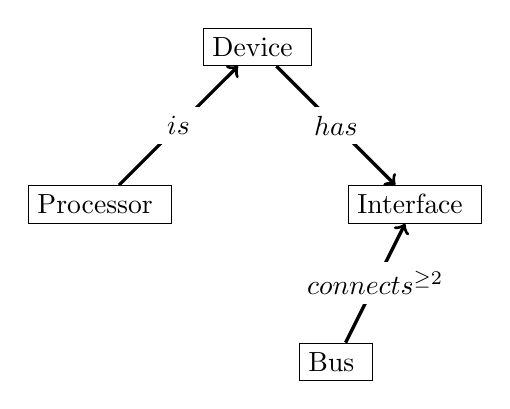
\begin{tikzpicture}
        \node[draw, align=center] (Device) at (1,0.5) {
            Device
        };
        \node[draw, align=center] (Processor) at (-1,-1.5) {
            Processor
        };
        %\node[draw, align=center] (Memory) at (3,2.5) {
        %    Memory
        %};
        %\node[draw, align=center] (Peripheral) at (1,-1.5) {
        %    Peripheral
        %};
        \node[draw, align=center] (Interface) at (3,-1.5) {
            Interface
        };
        \node[draw, align=center] (Bus) at (2,-3.5) {
            Bus
        };
        %\node[align=center] (contains) at (4,0.5) {
        %    $contains$
        %};
        \draw[->, very thick] (Device) to node[fill=white] {
            $has$
        } (Interface);
        \draw[->, very thick] (Processor) to node[fill=white] {
            $is$
        } (Device);
        %\draw[->, very thick] (Memory) to node[fill=white] {
        %    $is$
        %} (Device);
        %\draw[->, very thick] (Peripheral) to node[fill=white] {
        %    $is$
        %} (Device);
        \draw[->, very thick] (Bus) to node[fill=white] {
            $connects^{\geq 2}$
        } (Interface);
        %\draw[-, very thick] (Device) to [out=-45, in=-135] (contains);
        %\draw[->, very thick] (contains) to [out=135, in=45] (Device);
    \end{tikzpicture}
    \caption{
        Overview of the main aspects of the device model representing the computational hardware domain.
    }
    \label{fig:hw_new}
\end{figure}
The main entity in the hardware domain is the device.
Figure~\ref{fig:hw_new} denotes the relationships between device, interfaces and busses.
The subclasses except for the processors have been neglected.

% Traversals, Queries and Transitive Closure
A general graph traversal function has been implemented using breadth-first search and the visitor pattern to allow
\begin{itemize}
    \item the result set to be filtered according to a lambda function having signature bool(Hyperedge X), and
    \item the successor/predecessor set to be filtered according to a lambda function having signature bool(Hyperedge current, next).
\end{itemize}
This traversal is used to generate a new hyperedge representing the result of the query.
With this functionality transitive closure of the already introduced relations can be achived.
For example, following the \emph{isA} relation chain, a new \emph{isA} relation can be generated given the transitive property.

% Unique IDs
Every hyperedge and derived concept can have the same label/name.
This is possible because every edge gets assigned a unique id which is also used in the incidence lists of the edges.

% Serialization/Deserialization <- CURRENT STATE
Hyperedges and hypergraphs can be stored and retrieved using a YAML import/export class.
It is ensured that the result is valid even if parts of the system already exist.
In the future this functionality shall be used together with the GIT versioning system to allow the safe and consistent storage of evolving hypergraphs.

% Hyperedges \& GIT as DB || LMDB as backend
% Examples
% GUI
% Generators
% Mapping
% Results
\section{Preliminary Results}

% Outlook \& Discussion
\section{Outlook}

\end{document}
